\documentclass[tikz, border=4pt]{standalone}
\usepackage{amsmath,amssymb}
\usetikzlibrary{arrows.meta,positioning,shapes.geometric,fit,calc}
\usepackage{xcolor}

\definecolor{cblue}{RGB}{37, 99, 235}
\definecolor{cbluebg}{RGB}{245, 248, 255}
\definecolor{cteal}{RGB}{13, 148, 136}
\definecolor{ctealbg}{RGB}{240, 253, 250}
\definecolor{cpurple}{RGB}{109, 40, 217}
\definecolor{cpurplebg}{RGB}{248, 245, 255}
\definecolor{cgreen}{RGB}{22, 163, 74}
\definecolor{cgreenbg}{RGB}{240, 253, 244}
\definecolor{camber}{RGB}{217, 119, 6}
\definecolor{camberbg}{RGB}{254, 243, 199}
\definecolor{cred}{RGB}{220, 38, 38}
\definecolor{credbg}{RGB}{254, 242, 242}
\definecolor{cslate}{RGB}{100, 116, 139}

\begin{document}

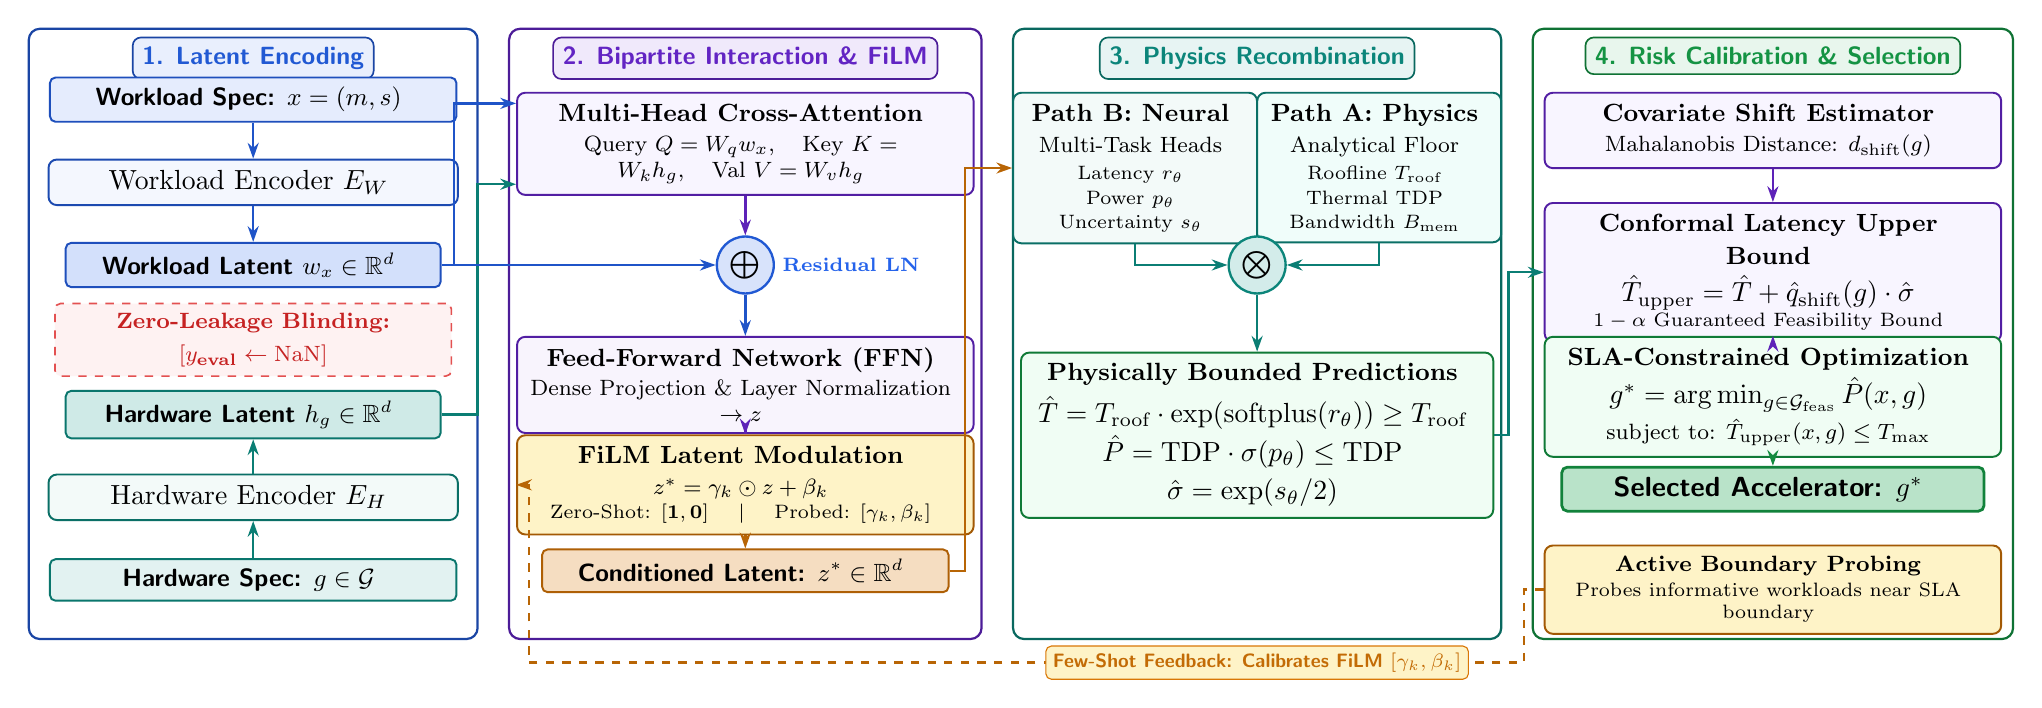
\begin{tikzpicture}[
    x=1.0cm, y=1.0cm,
    >=Stealth,
    container/.style={
        draw=#1!70!black,
        fill=white,
        line width=0.8pt,
        rounded corners=4pt
    },
    coltag/.style={
        draw=#1!70!black,
        fill=#1!10,
        line width=0.6pt,
        rounded corners=3pt,
        font=\sffamily\bfseries\small,
        text=#1!90!black,
        inner sep=3.5pt
    },
    block/.style={
        draw=#1!75!black,
        fill=#1!5,
        line width=0.7pt,
        rounded corners=3pt,
        align=center,
        inner sep=4pt
    },
    tensor/.style={
        draw=#1!80!black,
        fill=#1!12,
        line width=0.7pt,
        rounded corners=2pt,
        align=center,
        font=\sffamily\bfseries\small,
        inner sep=3.5pt
    },
    op/.style={
        draw=#1!90!black,
        fill=#1!18,
        circle,
        line width=0.85pt,
        align=center,
        font=\bfseries\normalsize,
        inner sep=2pt
    },
    arrow/.style={
        -{Stealth[length=2.0mm,width=1.4mm]},
        line width=0.85pt,
        draw=#1!85!black
    },
    dasharrow/.style={
        -{Stealth[length=2.0mm,width=1.4mm]},
        line width=0.85pt,
        dashed,
        draw=#1!85!black
    }
]

% ==============================================================================
% 1. LATENT ENCODING (X: 0.0 to 5.7)
% ==============================================================================
\draw[container=cblue] (0.0, 0.45) rectangle (5.7, 8.2);
\node[coltag=cblue, anchor=north] at (2.85, 8.1) {1. Latent Encoding};

% Workload Spec & Encoder
\node[tensor=cblue] (win) at (2.85, 7.3) {
    \parbox{4.8cm}{\centering Workload Spec: $x = (m, s)$}
};

\node[block=cblue] (wenc) at (2.85, 6.25) {
    \parbox{4.8cm}{\centering Workload Encoder $E_W$}
};
\draw[arrow=cblue] (win) -- (wenc);

\node[tensor=cblue, fill=cblue!20] (wlat) at (2.85, 5.2) {
    \parbox{4.4cm}{\centering Workload Latent $w_x \in \mathbb{R}^d$}
};
\draw[arrow=cblue] (wenc) -- (wlat);

% Zero-Leakage Blinding
\node[draw=cred!80, fill=credbg, dashed, line width=0.6pt, rounded corners=2pt] (blind) at (2.85, 4.25) {
    \parbox{4.8cm}{\centering \textcolor{cred!90!black}{\textbf{\footnotesize Zero-Leakage Blinding: $[y_{\text{eval}} \leftarrow \mathrm{NaN}]$}}}
};

% Hardware Latent & Encoder
\node[tensor=cteal, fill=cteal!20] (hlat) at (2.85, 3.3) {
    \parbox{4.4cm}{\centering Hardware Latent $h_g \in \mathbb{R}^d$}
};

\node[block=cteal] (henc) at (2.85, 2.25) {
    \parbox{4.8cm}{\centering Hardware Encoder $E_H$}
};
\draw[arrow=cteal] (henc) -- (hlat);

\node[tensor=cteal] (hin) at (2.85, 1.2) {
    \parbox{4.8cm}{\centering Hardware Spec: $g \in \mathcal{G}$}
};
\draw[arrow=cteal] (hin) -- (henc);

% ==============================================================================
% 2. BIPARTITE INTERACTION & FiLM (X: 6.1 to 12.1)
% ==============================================================================
\draw[container=cpurple] (6.1, 0.45) rectangle (12.1, 8.2);
\node[coltag=cpurple, anchor=north] at (9.1, 8.1) {2. Bipartite Interaction \& FiLM};

% Multi-Head Bipartite Attention Block
\node[block=cpurple, fill=cpurplebg, anchor=north] (attn) at (9.1, 7.4) {
    \parbox{5.4cm}{\centering \textbf{\small Multi-Head Cross-Attention}\\[0.15em]
    \footnotesize Query $Q = W_q w_x, \quad \text{Key } K = W_k h_g, \quad \text{Val } V = W_v h_g$}
};

% Purely Orthogonal Routing into Attention
\draw[arrow=cblue] (wlat.east) -- (5.4, 5.2) |- (attn.170);
\draw[arrow=cteal] (hlat.east) -- (5.7, 3.3) |- (attn.190);

% Residual Addition & LayerNorm (Horizontally aligned with wlat at Y=5.2)
\node[op=cblue] (add1) at (9.1, 5.2) {$\bigoplus$};
\node[font=\bfseries\scriptsize, cblue, anchor=west] at (9.45, 5.2) {Residual LN};
\draw[arrow=cpurple] (attn.south) -- (add1.north);
\draw[arrow=cblue] (5.4, 5.2) -- (add1.west);

% Feed-Forward Network
\node[block=cpurple, anchor=north] (ffn) at (9.1, 4.3) {
    \parbox{5.4cm}{\centering \textbf{\small Feed-Forward Network (FFN)}\\[0.1em]
    \footnotesize Dense Projection \& Layer Normalization $\to z$}
};
\draw[arrow=cblue] (add1.south) -- (ffn.north);

% FiLM Modulation Block
\node[block=camber, fill=camberbg, anchor=north] (film) at (9.1, 3.05) {
    \parbox{5.4cm}{\centering \textbf{\small FiLM Latent Modulation}\\[0.15em]
    \footnotesize $z^* = \gamma_k \odot z + \beta_k$\\[0.1em]
    \scriptsize Zero-Shot: $[\mathbf{1}, \mathbf{0}]$ $\quad\mid\quad$ Probed: $[\gamma_k, \beta_k]$}
};
\draw[arrow=cpurple] (ffn.south) -- (film.north);

% Conditioned Representation Tensor
\node[tensor=camber, fill=camber!25, anchor=north] (zfilm) at (9.1, 1.6) {
    \parbox{4.8cm}{\centering Conditioned Latent: $z^* \in \mathbb{R}^d$}
};
\draw[arrow=camber] (film.south) -- (zfilm.north);

% ==============================================================================
% 3. DUAL-PATH PHYSICS (X: 12.5 to 18.7)
% ==============================================================================
\draw[container=cteal] (12.5, 0.45) rectangle (18.7, 8.2);
\node[coltag=cteal, anchor=north] at (15.6, 8.1) {3. Physics Recombination};

% Path B: Neural Latent Heads (Left)
\node[block=cteal, anchor=north] (heads) at (14.05, 7.4) {
    \parbox{2.7cm}{\centering \textbf{\small Path B: Neural}\\[0.2em]
    \footnotesize Multi-Task Heads\\[0.2em]
    \scriptsize Latency $r_\theta$\\[0.1em]
    \scriptsize Power $p_\theta$\\[0.1em]
    \scriptsize Uncertainty $s_\theta$}
};
\draw[arrow=camber] (zfilm.east) -| ++(0.2, 0) |- (heads.west);

% Path A: Roofline Analytical Floor (Right)
\node[block=cteal, fill=ctealbg, anchor=north] (roof) at (17.15, 7.4) {
    \parbox{2.7cm}{\centering \textbf{\small Path A: Physics}\\[0.2em]
    \footnotesize Analytical Floor\\[0.2em]
    \scriptsize Roofline $T_{\text{roof}}$\\[0.1em]
    \scriptsize Thermal $\mathrm{TDP}$\\[0.1em]
    \scriptsize Bandwidth $B_{\text{mem}}$}
};

% Multiplicative Floor Operator (Centered cleanly between Path A & B)
\node[op=cteal, font=\bfseries\normalsize] (mult) at (15.6, 5.2) {$\bigotimes$};
\draw[arrow=cteal] (heads.south) |- (mult.west);
\draw[arrow=cteal] (roof.south) |- (mult.east);

% Physically Bounded Predictions Card
\node[block=cgreen, fill=cgreenbg, anchor=north] (preds) at (15.6, 4.1) {
    \parbox{5.6cm}{
        \centering
        \textbf{\small Physically Bounded Predictions}\\[0.3em]
        \normalsize
        $\hat{T} = T_{\text{roof}} \cdot \exp(\mathrm{softplus}(r_\theta)) \ge T_{\text{roof}}$\\[0.2em]
        $\hat{P} = \mathrm{TDP} \cdot \sigma(p_\theta) \le \mathrm{TDP}$\\[0.2em]
        $\hat{\sigma} = \exp(s_\theta / 2)$
    }
};
\draw[arrow=cteal] (mult.south) -- (preds.north);

% ==============================================================================
% 4. RISK CALIBRATION & SELECTION (X: 19.1 to 25.2)
% ==============================================================================
\draw[container=cgreen] (19.1, 0.45) rectangle (25.2, 8.2);
\node[coltag=cgreen, anchor=north] at (22.15, 8.1) {4. Risk Calibration \& Selection};

% Covariate Shift Metric
\node[block=cpurple, fill=cpurplebg, anchor=north] (maha) at (22.15, 7.4) {
    \parbox{5.4cm}{\centering \textbf{\small Covariate Shift Estimator}\\[0.15em]
    \footnotesize Mahalanobis Distance: $d_{\text{shift}}(g)$}
};

% Conformal Bound
\node[block=cpurple, fill=cpurplebg, anchor=north] (conf) at (22.15, 6.0) {
    \parbox{5.4cm}{\centering \textbf{\small Conformal Latency Upper Bound}\\[0.15em]
    \normalsize $\hat{T}_{\text{upper}} = \hat{T} + \hat{q}_{\text{shift}}(g) \cdot \hat{\sigma}$\\[0.1em]
    \scriptsize $1-\alpha$ Guaranteed Feasibility Bound}
};
\draw[arrow=cpurple] (maha) -- (conf);
\draw[arrow=cteal] (preds.east) -| ++(0.18, 0) |- (conf.west);

% Feasible Set & Optimization
\node[block=cgreen, fill=cgreenbg, anchor=north] (sel) at (22.15, 4.3) {
    \parbox{5.4cm}{
        \centering
        \textbf{\small SLA-Constrained Optimization}\\[0.2em]
        \normalsize $g^* = \arg\min_{g \in \mathcal{G}_{\text{feas}}} \hat{P}(x, g)$\\[0.15em]
        \footnotesize subject to: $\hat{T}_{\text{upper}}(x, g) \le T_{\max}$
    }
};
\draw[arrow=cpurple] (conf) -- (sel);

% Optimal Dispatch Output Node
\node[tensor=cgreen, fill=cgreen!30, line width=1.0pt, anchor=north] (out) at (22.15, 2.65) {
    \parbox{5.0cm}{\centering \normalsize \textbf{Selected Accelerator: $g^*$}}
};
\draw[arrow=cgreen, line width=1.2pt] (sel) -- (out);

% ==============================================================================
% BOTTOM ACTIVE PROBING LOOP: Clean Abstract Arrow
% ==============================================================================
\node[block=camber, fill=camberbg, anchor=north] (roaa) at (22.15, 1.65) {
    \parbox{5.4cm}{\centering \textbf{\footnotesize Active Boundary Probing}\\[0.1em]
    \scriptsize Probes informative workloads near SLA boundary}
};
\draw[dasharrow=camber] (roaa.west) -- ++(-0.25, 0) |- (15.6, 0.15) -- (6.35, 0.15) |- (film.west);
\node[fill=camberbg, draw=camber, rounded corners=2pt, font=\sffamily\bfseries\scriptsize, text=camber!90!black, inner sep=2.5pt] 
    at (15.6, 0.15) {Few-Shot Feedback: Calibrates FiLM $[\gamma_k, \beta_k]$};

\end{tikzpicture}

\end{document}
